\chapter{Astrophysical applications}
\label{c:astrophysical-applications}
\section{Triaxial blast wave}\label{Ellipsoid blast wave test}
This triaxial relativistic blast wave problem models a hypothetical astrophysical mega-explosion driven by an ultra-relativistically hot plasma source absent of particular symmetry. It is an atypical test for which we verify the code's ability to deal with strong 3D shocks. The simulation evolves a blast wave from a triaxial source in a homogeneous medium. The triaxial source has aspect ratios $1:1.5:2$ with a semi-major axis $0.01L$ aligned with the diagonal direction, where $L$ is the width of a cubic computational box. The source is filled with a uniform ultra-relativistic ($k_{B}T_{\text{src}}/mc^2=10^{6}$) plasma and the ambient is filled with a uniform non-relativistic ($k_{B}T_{\text{amb}}/mc^2=10^{-9}$) HII gas. The density is homogeneous throughout the entire domain with $\rho_{\text{src}}=\rho_{\text{amb}}=1.0$. After the system quickly relaxes, the hot plasma rapidly expands driving a forward shock traveling almost at the speed of light.

The AMR base level is covered by $32^3$ cells with the periodic boundary condition. The highest refinement level is 9 so that the initial source can be adequately resolved by approximately 82 cells along the minor axis. To refine both the initial source and the thin shell of the blast wave shock, we adopt the gradient of the reduced energy density as the refinement criterion, with $Q=\tilde{E}$ and $C_{Q}=1.0$ in \Cref{threshold for gradient}.

For comparison, we also simulate a spherical blast wave to understand how the initially triaxial shape affects the evolution of the ultra-relativistic blast wave. Both the spherical and triaxial cases have the same simulation set-up and the same source volume, i.e. $r/L=\sqrt[3]{0.01\times0.0075\times0.005}$, where $r$ is the radius of the spherical source.

\Cref{fig:Ellipsoid blast wave} shows the results. We observe that the interior hot plasma pushes out a contact discontinuity immediately inward of the shock and that the thickness of the shell between the contact discontinuity and the shock diminishes in time. In early time, the triaxial profiles ($\MyCross[draw=BlastTriNew,fill=BlastTriNew]$) at $t=0.05L/c$ deviate from the spherical counterparts ($\MySolidLine[draw=BlastSphNew,fill=BlastSphNew]$), especially in the pressure and proper mass density, although the shock positions almost coincide. However, at a later time, the profiles at $t=0.3L/c$ show no significant difference between the triaxial ($\tikz\draw[BlastTriOld,fill=BlastTriOld,line width=1] (0,0) circle (.5ex);$) and spherical ($\MySolidLine[draw=BlastSphOld,fill=BlastSphOld]$) blast waves, indicating the initial shape of the source does not have a great impact on the asymptotic evolution of ultra-relativistic blast waves.

To further investigate how the triaxial blast wave evolves into a spherical one, we extract the radii $R_{L}(t)$ and $R_{S}(t)$ of the triaxial blast wave along the semi-major ($r_{L}$) and semi-minor axes ($r_{S}$) of the initial source from simulation data. As shown in \Cref{fig:BlastFitting}, we find that the dimensionless quantity $\left(\ln \left(\left(\frac{R_{L}-R_{S}}{\sqrt{R_{L}R_{S}}}\right)/ \left(\frac{r_{L}-r_{S}}{\sqrt{r_{L}r_{S}}}\right)\right)\right)^{2}$ is approximately equal to $0.66\left(\sqrt{R_{L}R_{S}}/\sqrt{r_{L}r_{S}}-1\right)$. This dependence suggests that the triaxiality is damped out with the blast wave propagation by the relation:
\begin{equation}
\begin{aligned}
          &\frac{R_{L}(t)-R_{S}(t)}{\sqrt{R_{L}(t)R_{S}(t)}} =\\ &\left(\frac{r_{L}-r_{S}}{\sqrt{r_{L}r_{S}}}\right)\text{exp}\left[-0.81\left(\frac{\sqrt{R_{L}(t)R_{S}(t)}}{\sqrt{r_{L}r_{S}}}-1\right)^{1/2}\right].
\end{aligned}
\label{eq:FittingBlast}
\end{equation}

We remark that this test problem also demonstrates that \textsc{gamer-sr} can successfully handle ultra-relativistic gases embedded in a cold HII region, which can be difficult for conventional SRHD codes.

\begin{figure*}
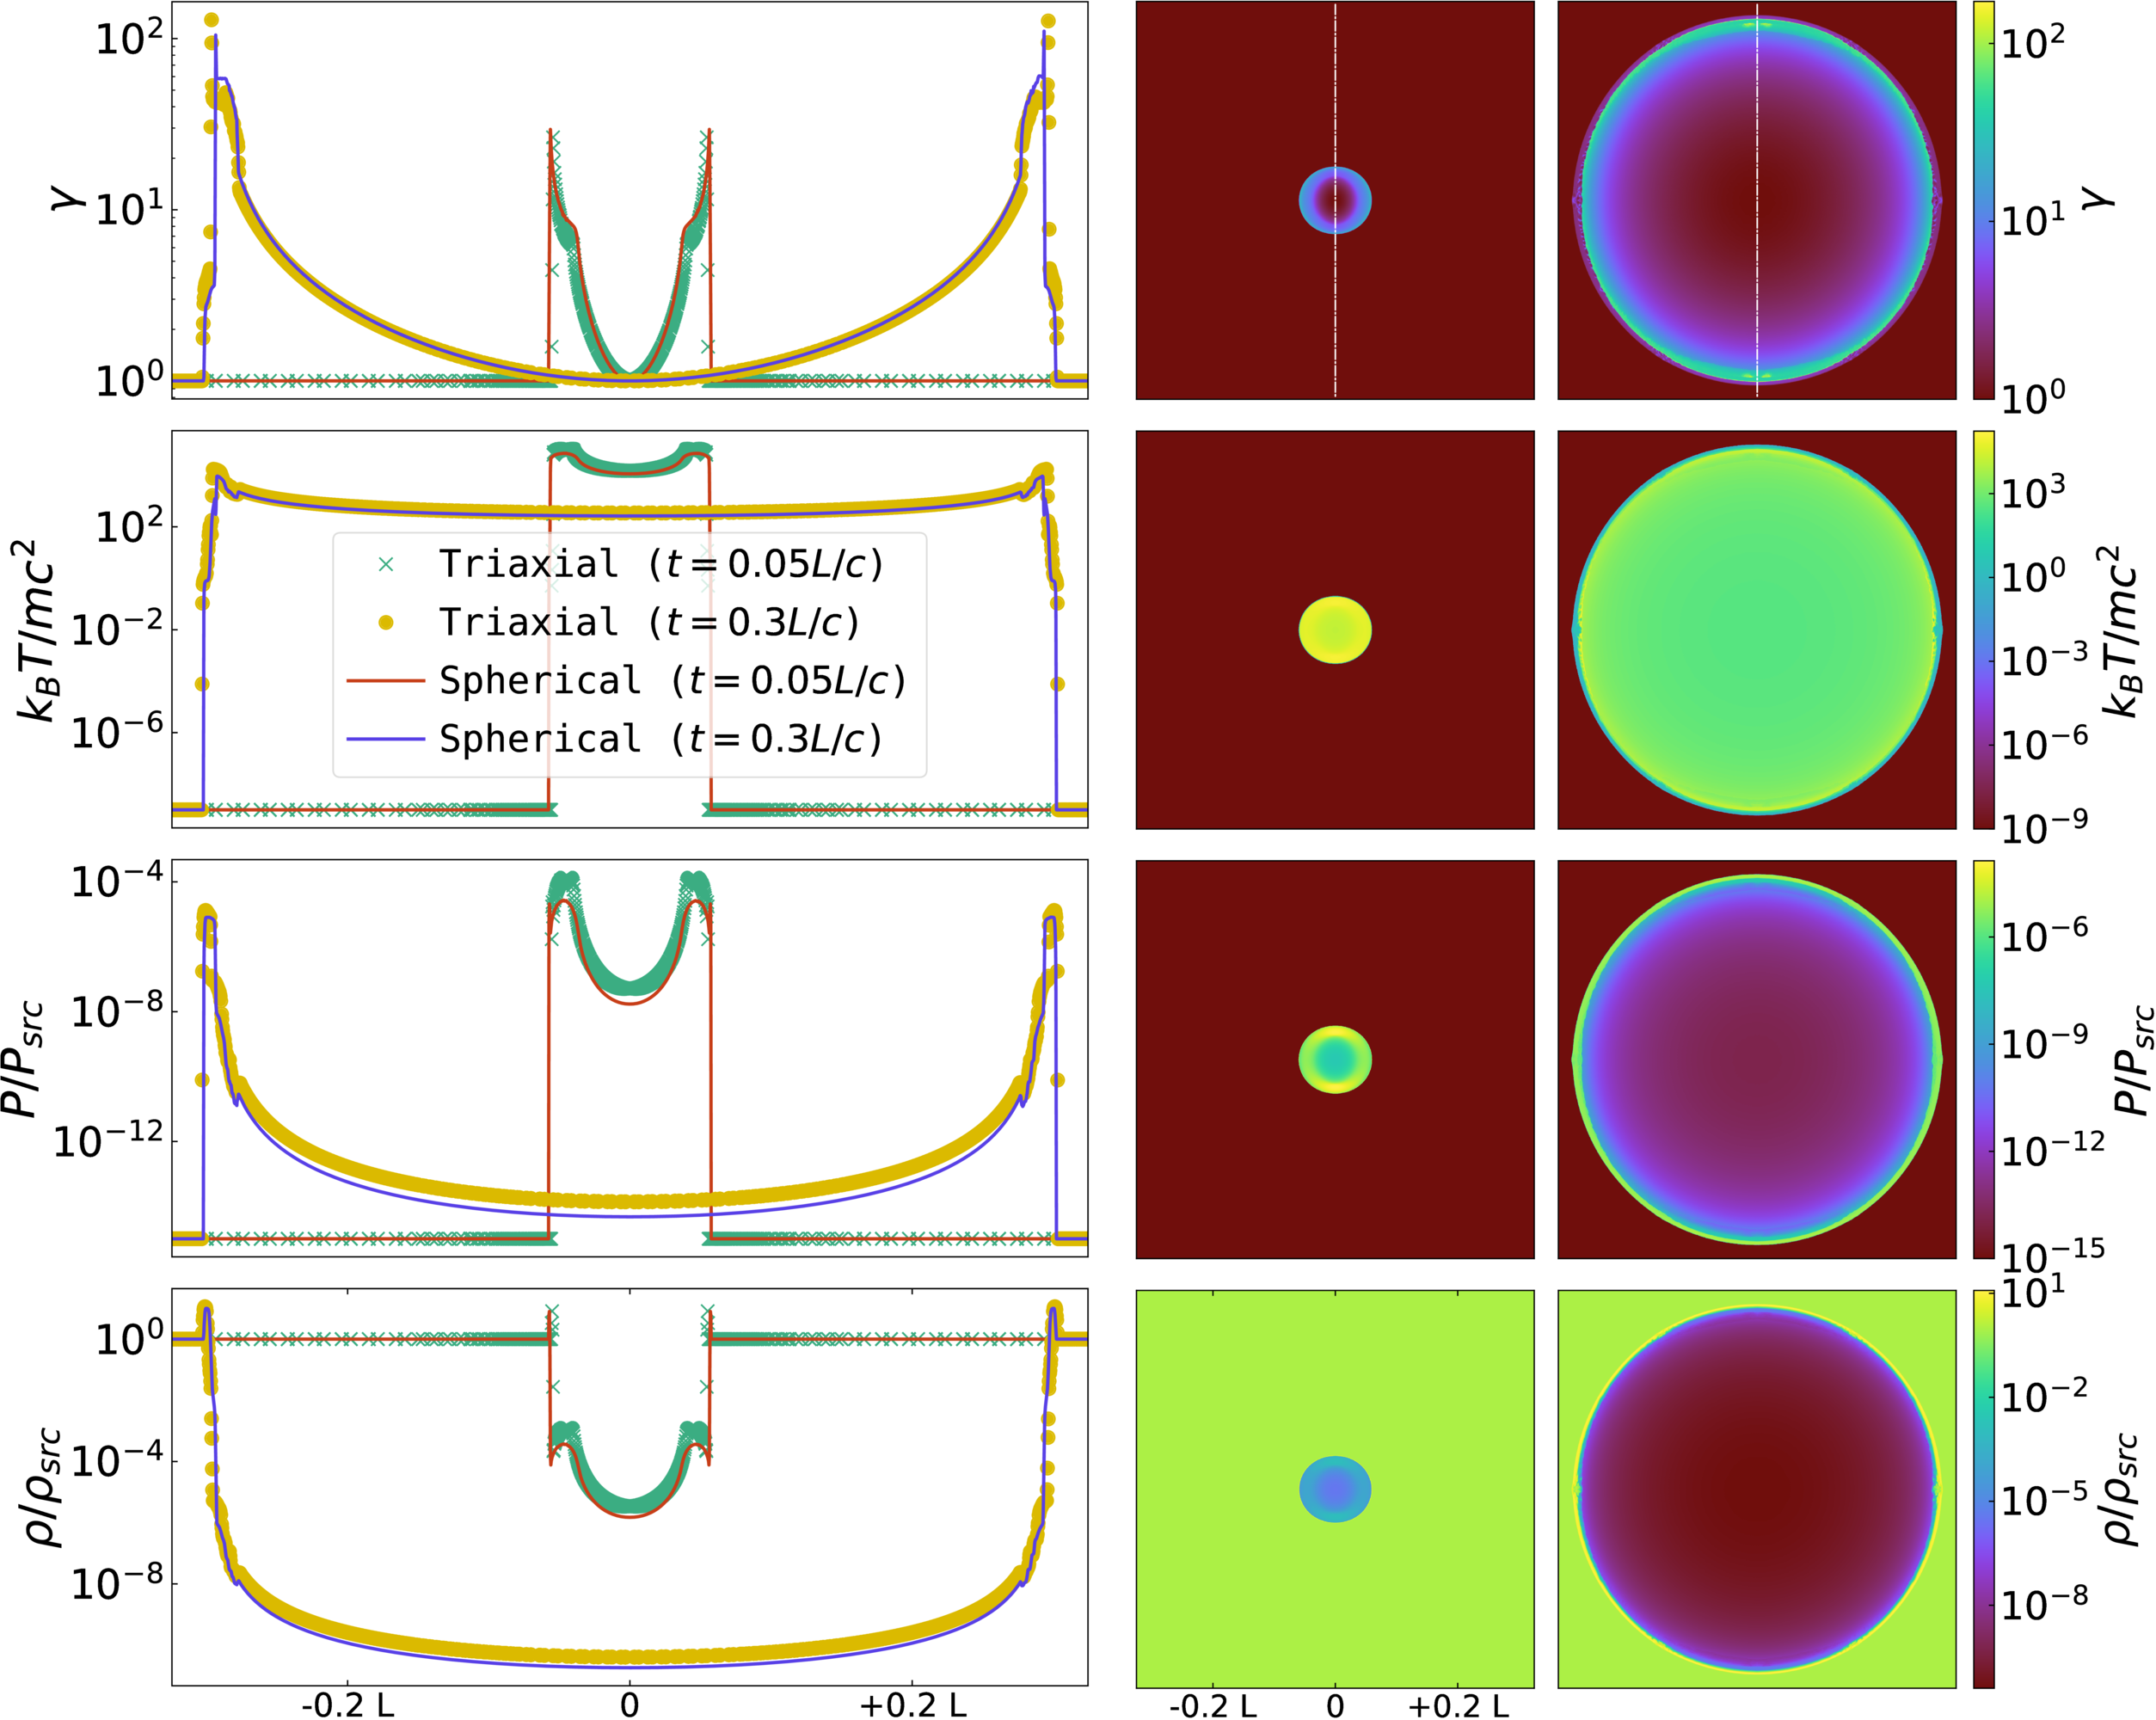
\includegraphics[width=\linewidth]{srhd-figures/ProfileSliceLowRes.png}
\centering
\caption{Triaxial blast wave test. The middle ($t=0.05L/c$) and right ($t=0.3L/c$) columns show the slices passing through the triaxial source at the mid-plane of its intermediate axis (i.e. the horizontal and vertical axes are along the major and minor axes, respectively). The left column shows the profiles along the minor-axis (i.e. the white dotted-dashed line in the $\gamma$ map).}
\label{fig:Ellipsoid blast wave}
\end{figure*}

\begin{figure}
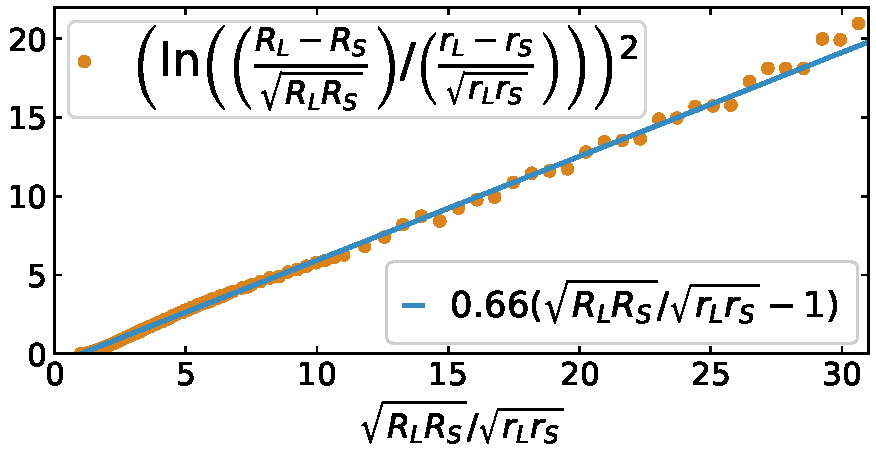
\includegraphics[width=\linewidth]{srhd-figures/fig__AxesRatio.pdf}
\caption{Damping of the triaxiality in the triaxial blast wave test, where $R_{L}$ and $R_{S}$ are the radii of the triaxial blast wave along the semi-major ($r_{L}$) and semi-minor axes ($r_{S}$) of the initial source.}
\label{fig:BlastFitting}
\end{figure}

\section{Limb-brightened jet}
\label{Limb-brightened jet}
Most active galactic nuclei (AGN) jets in VLBI observations appear ridge-brightened, while limb-brightened jets are rare and have been reported only in a few nearby radio galaxies, such as Mrk 501 \citep{Giroletti2004}, M87 (\citealt{Asada2012}; \citealt{Kim2018}), Cygnus A \citep{Boccardi2015}, and 3C84 (\citealt{Nagai_2014}; \citealt{Giovannini2018}). Motivated by these observations, we simulate a three-dimensional SRHD jet using \textsc{gamer-sr} to study its acceleration and collimation in the hope to shed light on the limb-brightened jets.

We adopt the gradient of the reduced energy density and the magnitude of $\abs{\mathbf{M}}/D$ as the two inclusive refinement criteria. A patch is refined if any cell satisfies either \Cref{threshold for gradient} with $Q=\tilde{E}$ and $C_{Q}=0.1$ or $\abs{\mathbf{M}}/D>20$. The first criterion aims to capture the strong terminal shock and the cocoon, while the second one ensures that the central `spine' region of the jet can be properly resolved.

The jet is continuously ejected from a cylindrical source with four-velocity $\beta\gamma=10.0$ ($\gamma \sim 10.05$). The proper mass density ratio between the jet source and the ambient gases is set to 1.0. The temperature ($k_{B}T/mc^2$) of the source and the ambient gases are set to 0.5 and $10^{-5}$, respectively. The outflow is thus an extremely under-pressured jet. Both the diameter and the length of the cylindrical source are well resolved by 32 cells.

\Cref{fig:Limb_brightened_jet} shows the simulation results. It demonstrates that the jet flow is entirely confined by a turbulent cocoon at all time. Two points are worth noting from these longitudinal slices. First, the Lorentz factor (first row) rises from $10$ to $26$, and meanwhile the temperature (second row) drops from 0.5 to 0.01 along the jet. Second, the relativistic Bernoulli number minus $c^2$ (fifth row), defined as $h\gamma-c^2$, remains nearly constant within the spine region. According to the de Laval nozzle effect, these suggest that thermal energy is converted to kinetic energy by the expansion of a supersonic flow. Surprisingly, the gases are still accelerated in the region between the label `C' and the confinement point close to `D'. These images seem to suggest acceleration during flow convergence, which in fact does not contradict the de Laval nozzle effect. The gases still expands away from the jet axis after passing `C', which can be confirmed by examining the transverse slice of the radial component of the Mach number (the last row),
\begin{equation}
     \mathscr{M}_{\text{radial}}=\left(\hat{r}\cdot \mathbf{U}\right)/\left(c_{s}\gamma_{s}\right),
     \label{eq:transverse Mach number}
 \end{equation}
where $\hat{r}$ is the cylindrical unit radial vector, $\mathbf{U}$ is the four-velocity of flow, and $\gamma_{s}=c_{s}/\sqrt{1-c_{s}^2}$. The definition of the radial Mach number given by \Cref{eq:transverse Mach number} is Lorentz invariant when the transforming direction is along the jet. Obviously, gases expand not only between the jet source and `C', but also inside the entire central spine region. Thus, the flow convergence in between `C' and `D' is a false impression.

Associated with this expanding jet flow is the limb-brightened phenomenon. Confined by the cocoon, the radial flow of the cooler jet imparts onto the cocoon with a boundary shock, as signified by the edge $\mathscr{M}_{\text{radial}} \gg 1$. Hot gases in the post-shock region then diffuse into the cocoon transverse to the jet through some instabilities composed of high-density and low-temperature fingers. This finger pattern is similar to that reported in Section \ref{Multi-dimensional grid effects}.

Certainly the boundary shock can generate particle acceleration and produce extra synchrotron brightness at the jet edge, thus yielding limb brightening. Since the boundary shock is relatively weak, the extra synchrotron brightness cannot be immense. This may explain why limb brightening is mostly observed in nearby AGN jets.

\begin{figure*}
	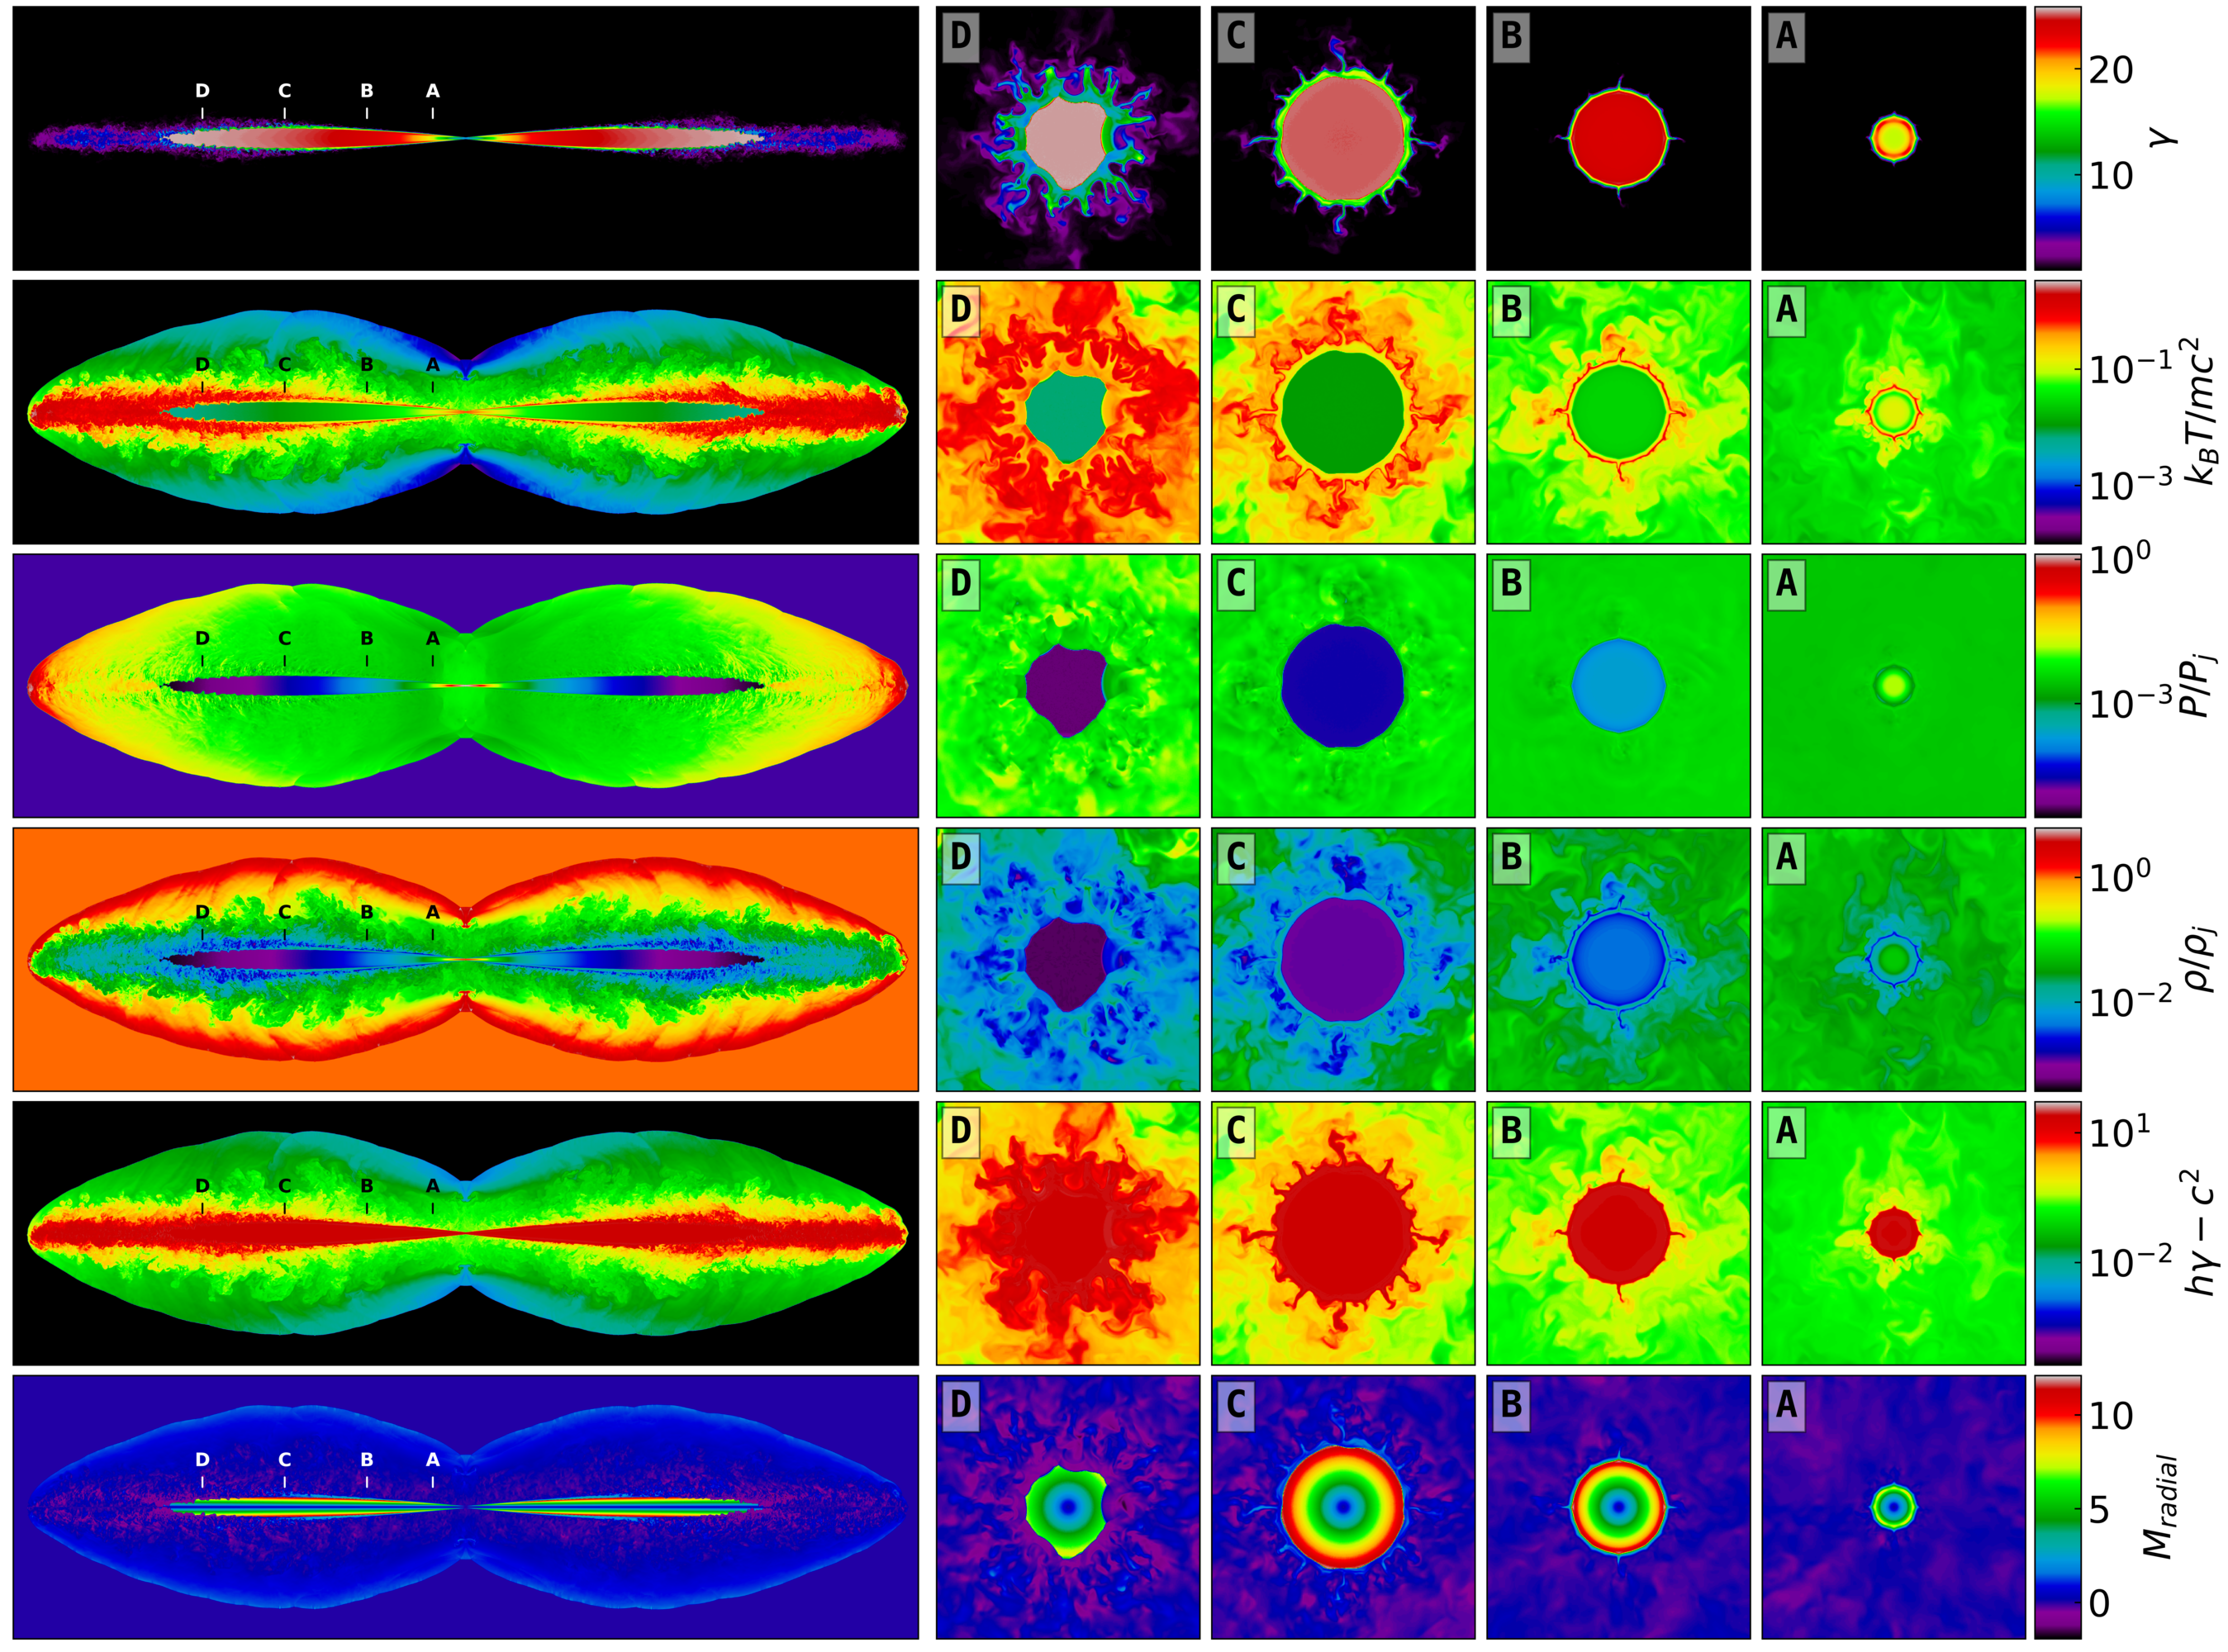
\includegraphics[width=\linewidth]{srhd-figures/JetAccLowRes.png}
    \caption{
    From top to bottom: Lorentz factor, temperature, pressure (normalized by the jet source pressure $p_{\text{j}}$), proper mass density (normalized by the jet source density $\rho_{\text{j}}$), relativistic Bernoulli number minus $c^2$ (i.e. $h\gamma-c^2$), and radial component of Mach number defined by \Cref{eq:transverse Mach number} at $t=0. 73 L/c$. Left column: longitudinal slices passing through the jet source. Right four columns: transverse slices passing through the locations labelled by A, B, C, and D.}
   \label{fig:Limb_brightened_jet}
\end{figure*}


